\chapter{Reconstruction}
The physics objects are reconstructed from the signals measured in the detector, and calibrated by the simulated events and observed data. 
The reconstruction and the calibration process in the current analysis is described in this chapter.

\section{Tracks and Vertices}
The track is reconstructed by the Inner Detector (ID). Reconstruction of tracks starts from three-dimentional space points, reconstructed from energy deposits of charged particles, in other words, cluster hits, in the ID components. The track candidate is formed with the sets of space points. The "track score" is calculated and tracks are selected with respect to the scores. Finally the track is fitted and decided. 
Details are described in \cite{PERF-2015-08}.
\section{Clusters}
The reconstruction of the signal from hadrons and jets is based on a three-dimensional topological clustering of individual calorimeter cell signals.
The cluster formation follows cell signal-significance patterns generated by electromagnetic and hadronic showers. 
In this, the clustering algorithm implicitly performs a topological noise suppression by removing cells with insignificant signals which are not in close proximity to cells with significant signals. These clusters are called Topo-clusters. Details are described in \cite{PERF-2014-07}.
%need more explanations?
\section{Electrons}
%reconstruction
Electron candidates are reconstructed from energy deposits (topological clusters) in the electromagnetic calorimeter (ECal), matched to a track identified by the inner detector. The associated track requirement in the inner detector is for distinguish electrons from photons. The electron track candidates are reconstructed, using an optimized algorithm to accout for the energy losses due to Bremsstrahlung radiation, then electron candidate are built by matching an electron-track candidate to a calorimeter seed cluster. The electron candidate is from the area up to $|\eta|<2.47$, excluding the transition region between barrel and endcap (1.37 < $|\eta|$ < 1.52).
%identification
The reconstructed electron is required the transverse energy of $E_T$ > 7~GeV and $|\eta|$ < 2.47. A likelihood-based identification (LHID) is required to reduce the backgrounds from leptons or hadron in jets. This LHID combines various identification variables, and electron candidates are categorized to LooseLH, MediumLH, and TightLH corresponding to 96\%, 94\%, 88\% of identification efficiencies to signal electrons at $E_T$ = 100~GeV, respectively.
%put calibration things here.....
The reconstruction and identification efficiency is measured using  $J/\Phi \rightarrow \e\e$ and $Z\rightarrow \e\e$ and $Z\rightarrow \e\e\gamma$ events. The difficiencies are shown in Figure~\ref{fig:recoElectron}. The discrepancy between the data and the MC is corrected for using event-weight scale factors, parametrized with $E_T$ and $\eta$. Detailed information is in \cite{PERF-2017-01}.

\begin{figure}[tbp]
\begin{center}
%\subfigure[]{
 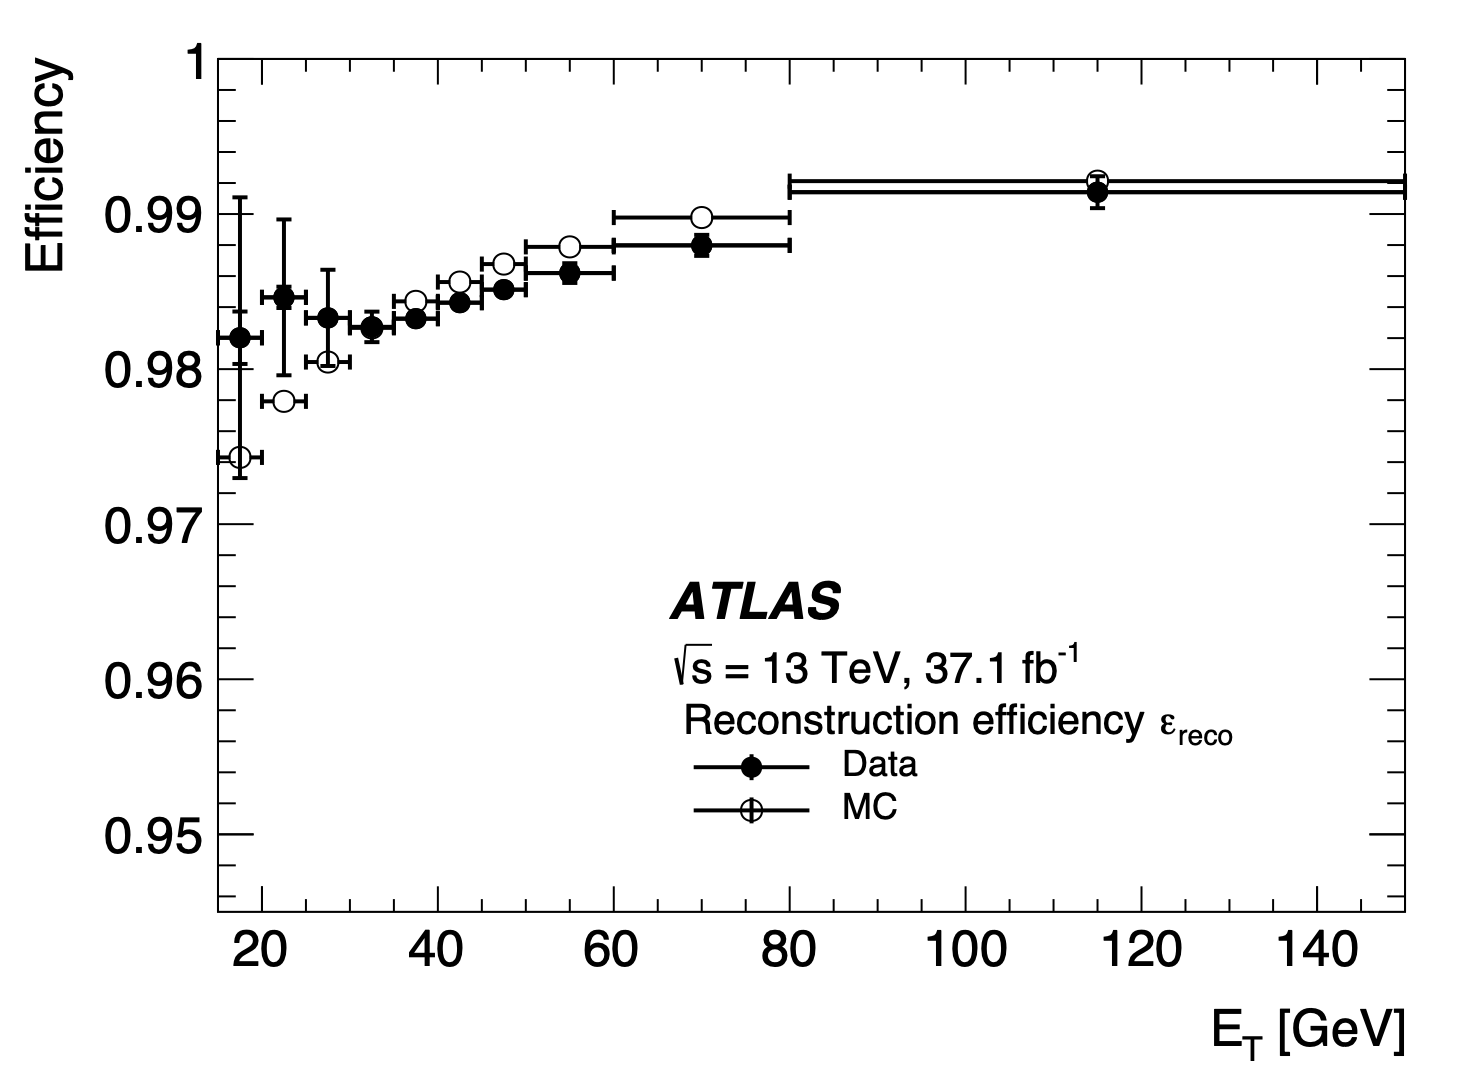
\includegraphics[width=0.50\textwidth,keepaspectratio]{figures/recoElectron}
%}
\caption{
electron reconstructing efficiency
}
\label{fig:recoElectron}
\end{center}
\end{figure}
Several furthermore requirement is applied for isolation, to reduce the contamination with jets. The two isolation working points used in this analysis, which are determined by the track and ECal informations, respectively. The selections applied in this analysis are shown in the Table~\ref{tab:electron_selection}.
Furthermore, the track related requirement is applied. $d_0$ is a minimum distance between the primary vertex (PV) and the track, and $\sigma_{d_0}$ is its uncertainty. $z_0$ is the tranverse impact parameter relative to the beamline.
\begin{table}[ht]
\resizebox{\textwidth}{!}{
\begin{tabular}[ht]{|l|c|c|c|}
  \hline
  & \emph{Loose} & \emph{Tight}\\
  \hline
  \hline
  $p_T$ & 7~GeV & 30~GeV\\
  \hline
  $|\eta|$ & \multicolumn{2}{c|}{$|\eta| < 2.47$ \notin [1.37,1.52]} \\
  \hline
  Identification & LooseLH & TightLH \\
  \hline
  Isolation &  FCLoose $(p_T <100~GeV)$                   &  FixedCutHighPtCaloOnly \\
            &  no isolation requirement $( >100~GeV )$ & \\
  \hline
  $|d_{0}/\sigma_{d_0}|$ & \multicolumn{2}{c|}{ <~5 }\\ 
  \hline
  $| z_{0} \sin{\theta}|$ & \multicolumn{2}{c|}{ <~0.5~mm }\\
  \hline
 \end{tabular}}
 \label{tab:electron_selection}
 \caption{Summary of electron selection used in this analysis}
\end{table}

\section{Muons}
%reconstruction
Muon is reconstructed by the combination of the tracks in the Inner Detector (ID) and Muon Spectrometer (MS). Several algorithm are used for the reconstruction: combined (CB) muons which require independent tracks both in ID and the MS. VB muons are of highest quality, but least acceptance. Segment-tagged (ST) muons require an ID track with only one hit in the MS, which allows recovering the low-$p_T$ muons. Calorimeter-tagged (CT) muon is reconstructed by requiring one ID track and in addition energy deposits in the calorimeter, which agree with a minimum-ionizing particle. CT muon are used to increase the acceptance in the region of $|\eta| < 0.1$, where the region without the muon cells due to the layout of the calorimeter cables. 
%reconstruction efficiency of calibration things
The muon reconstruction efficiency is measured with sample of $J/\Phi \rightarrow \mu\mu$ and $Z\rightarrow \mu\mu$, as well as the momentum scale and resolution.
The reconstruction efficiency is measured to be close to 99\% over most of the covered phase space ($|\eta|$ < 2.5 and 5 < $p_{T}$ < 100 GeV). The isolation efficiency varies between 93 and 100 \% depending on the selection applied and on the momentum of the muon. Both efficiencies are checked to be well reproduced in MC simulation. 
%In the central region of the detector, the momentum resolution is measured to be 1.7 \% (2.3 \%), and the momentum scale is known with an uncertainty of 0.05 \%. In the region $|\eta|$ > 2.2, the $p_T$ resolution for muons is 2.9 \% while the precision of the momentum scale for low-$p_T$ muons is about 0.2 \% \cite{}.
%identification
The further instructions are shown in \cite{MUON-2018-03}.
Similar to the electron, the isolation requirement is also applied to the muons, as shown in the Table~\ref{tab:muon_selection}.
\begin{figure}[tbp]
\begin{center}
%\subfigure[]{
 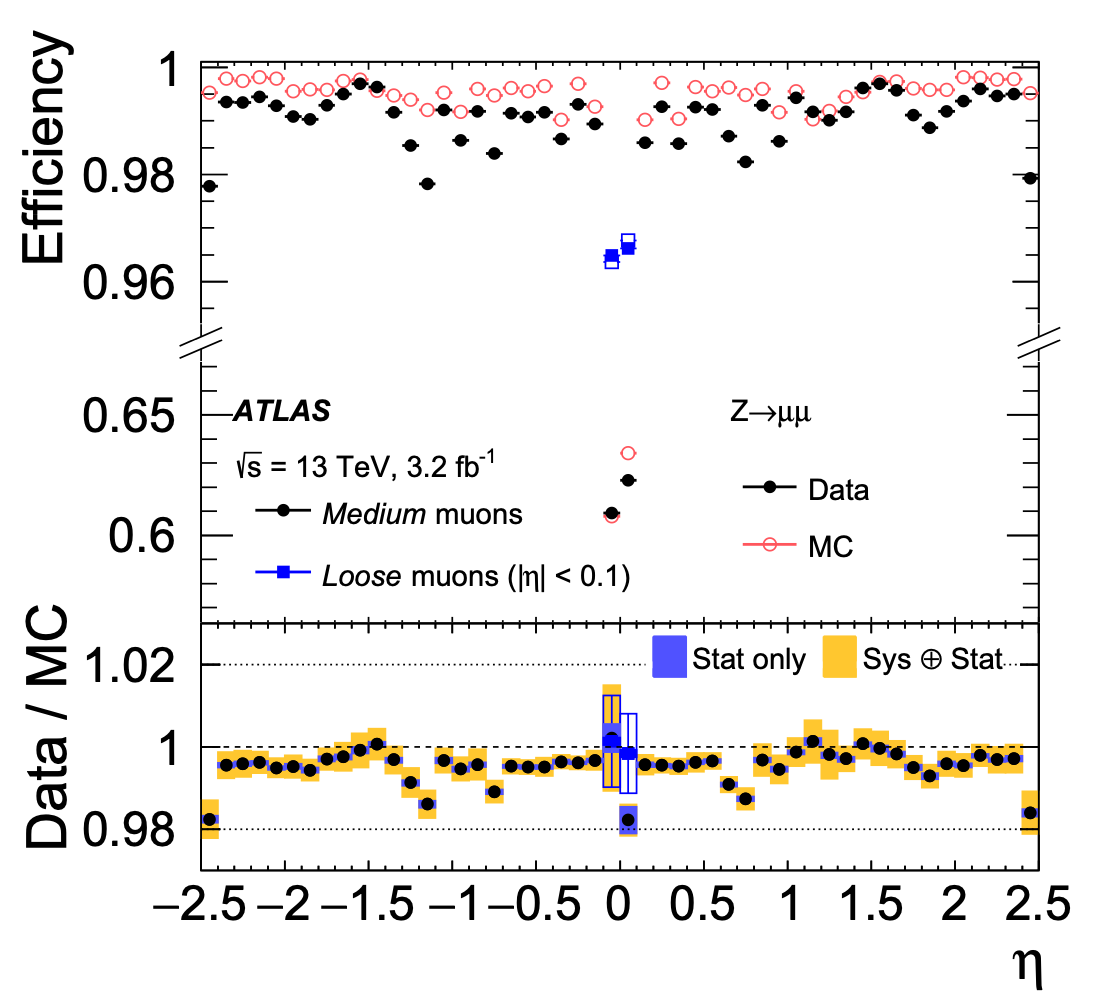
\includegraphics[width=0.50\textwidth,keepaspectratio]{figures/recoMuon}
%}
\caption{
muon reconstructing efficiency \cite{MUON-2018-03}
}
\label{fig:recoMuon}
\end{center}
\end{figure}
Muon identification is performed by applying quality requirements that suppress background, mainly from pion and kaon decays. 
%It also selects prompt muons with high efficiency and/or guaranteeing a robust momentum measurement. 
For Medium muons, the CB tracks required to have more than three hits in at least two MDT layers exept for |$\eta$|<0.1.
Specifically, the q/p significance is required to be less than seven for the contamination of the hadrons misidentified as muons.
The Loose identification uses all types of Muons. All CB and ME muons satisfying the Medium requirements are included. 
The identification used in this analysis is shown in Table~\ref{tab:muon_selection}.
\begin{table}[ht]
\resizebox{\textwidth}{!}{
\begin{tabular}[ht]{|l|c|c|c|}
  \hline
  & \emph{Loose} & \emph{Tight}\\
  \hline
  \hline
  $p_T$ & 7~GeV & 30~GeV\\
  \hline
  $|\eta|$ & \multicolumn{2}{c|}{$|\eta| < 2.5$} \\
  \hline
  Identification & Loose & Medium \\
  \hline
  Isolation &  FCLoose $(p_T <100~GeV)$                   &  FixedCutHighPtCaloOnly \\
            &  no isolation requirement $( >100~GeV )$ & \\
  \hline
  $|d_{0}/\sigma_{d_0}|$ & \multicolumn{2}{c|}{ <~3 }\\ 
  \hline
  $| z_{0} \sin{\theta}|$ & \multicolumn{2}{c|}{ <~0.5~mm }\\
  \hline
 \end{tabular}}
 \label{tab:muon_selection}
 \caption{Summary of muon selection used in this analysis}
\end{table}

\section{Jets}
Jets are basically reconstructed by grouping energy deposits in the calorimeter into clusters. These are then combined by the anti-$k_t$ algorithm \cite{Cacciari_2008}, with a radius of R = 0.4 (small-R jets) or R = 1.0 (large-R jets). 
There are two different types of reconstructed jets are used in this analysis for small-R jets and large-R jets.
\subsection{small-R Jets}
The small-R jets are reconstructed as so-called PFlow jets, by using particle flow algorithm \cite{PERF-2015-09}. These types of jets are reconstructed from the ensemble of signals from the calorimeter and the inner tracker. The topo-clusters using anti-$k_t$ algorithm are used.
\subsubsection{B-tagging}

\subsection{large-R Jets}
%%%%%%
\section{Missing Transverse Momentum}


